\section{Introduction}\label{sec:introduction}

Spatial and immersive audio techniques have been the beneficiaries of
significant research interest over the past few decades.
Recent developments in virtual and augmented reality technologies and
\textit{object-based} audio have led to an acceleration in interest in the
creation of virtual sound fields via approaches such as Wave Field Synthesis
(WFS) and Higher Order Ambisonics (HOA)~\citep{berkhout_acoustic_1993,
    ahrens_theory_2008,daniel_further_2003,frank_producing_2015}.
These techniques call for the deployment of large numbers of loudspeakers, and
centralised, \textit{in situ} installations of dedicated hardware and software.
The costs associated with such installations have seen them largely restricted
to the preserve of concert venues, cinemas, and institutions with the means to
purchase and operate large-scale systems of this sort.

Advancements in embedded computing mean that there now exist an assortment of
small, low-cost devices with support for audio digital signal processing (DSP).
These devices are open source, relatively easy to program, and may provide
support for communication over ubiquitous computer networking equipment and
protocols.
A network of such devices could be used to \textit{distribute} the problem of
audio spatialisation, potentially lowering the barrier to entry to what is
otherwise a comparatively exclusive branch of audio research.

%The work that this article describes is an exploration of the possibility of
%achieving such an outcome.
In this article \textemdash{} which is adapted from a master's thesis written by
the corresponding author, and builds on previous work on a microcontroler-based
networked audio client~\citep{rushton_microcontroller-based_2023} \textemdash{}
we describe the development of a distributed system for spatial and immersive
audio.


%This system is predicated, fundamentally, on the transmission of digital audio
%signals throughout a computer network.
%It is meaningful, then, to reflect on the nature of such signals, a selection
%of their properties of greatest pertinence to this work, and the representation
%of audio signals within computer systems and networks.

%\subsection{Digital Audio Signals}\label{subsec:digital-audio-signals}
%
%In a digital audio system with sampling rate $F_s$, an audio signal $y$ is
%composed of samples $y[n]$, each representing the amplitude of the signal at a
%given point in time $t$, where $t = n/F_s$.
%For arithmetical convenience, sample amplitudes are typically treated as
%floating point numbers, constrained to the interval $y \in [-1, 1]$ (see
%\figref{fig:signal-samples}).
%It is in this form that audio samples are typically handled during the
%processing stage of a DSP algorithm, and the underlying representation
%\textemdash{} that required by low level software and hardware systems
%\textemdash{} is concealed; matters of numerical resolution and precision are,
%by-and-large, abstracted away.
%
%\begin{figure}[ht]
%    \centering
%    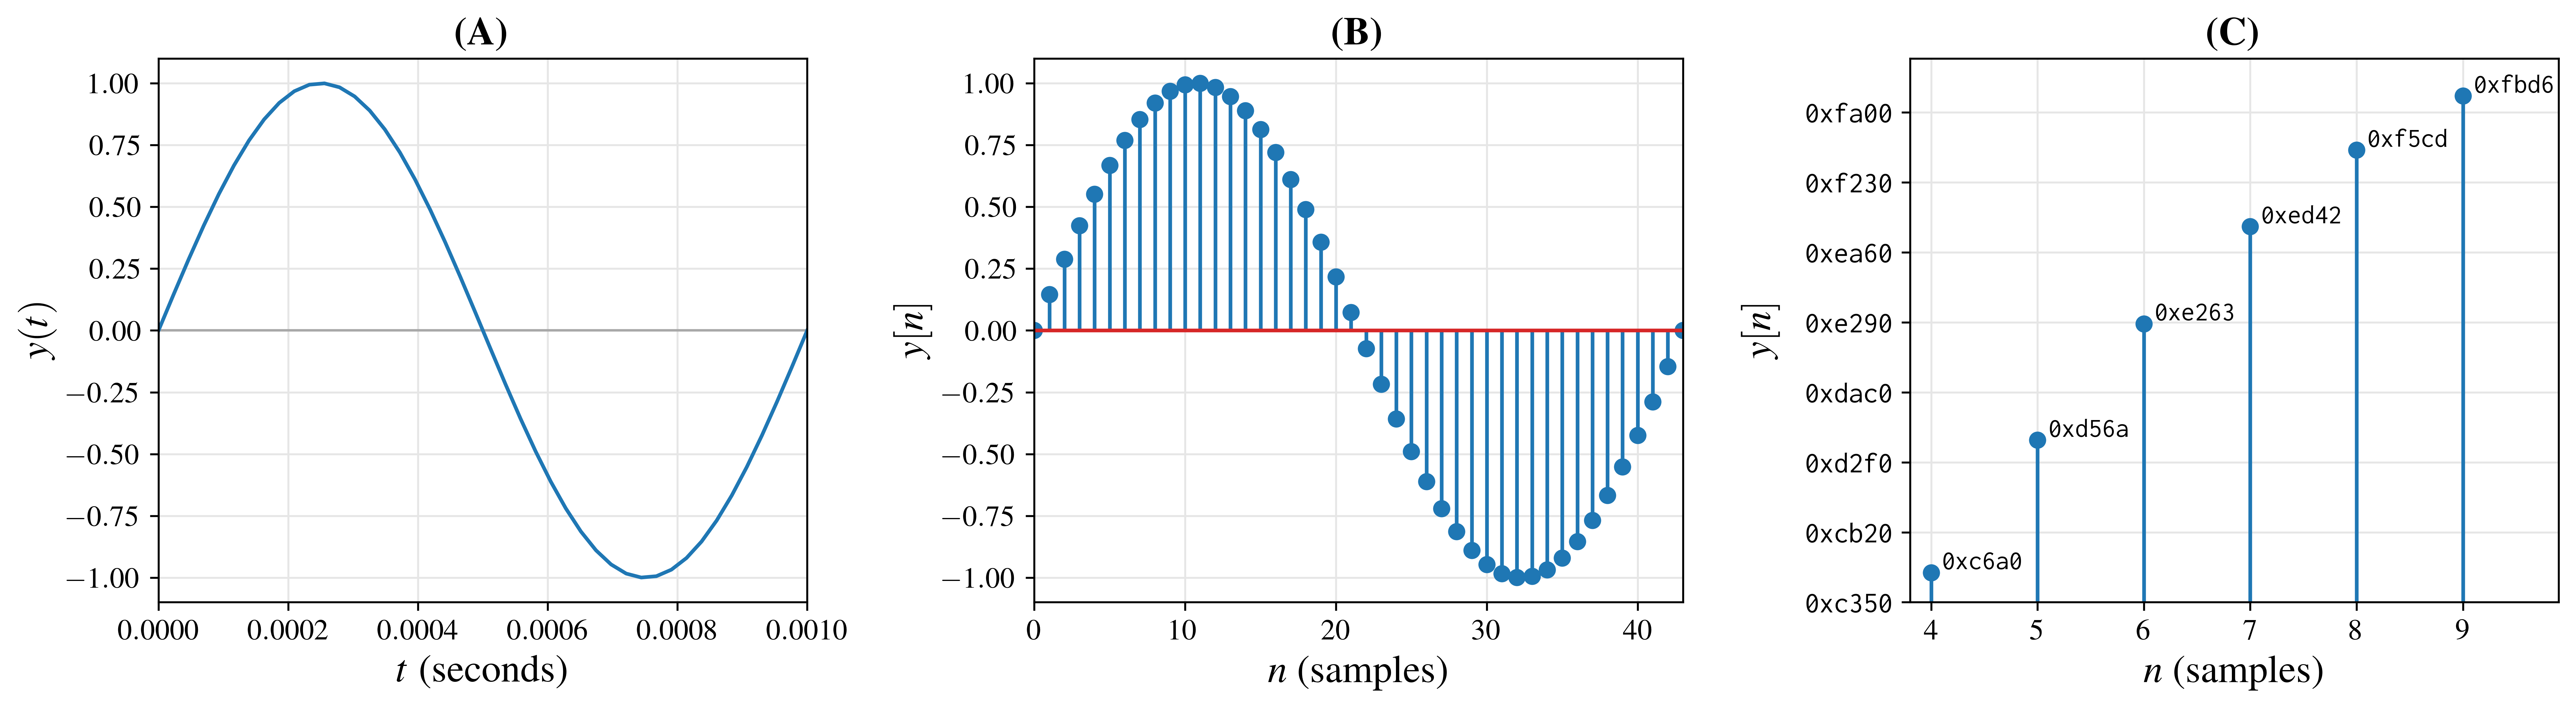
\includegraphics[width=\textwidth]{figures/digital-signal}
%    \caption{
%        An audio signal (\qty{1}{\kHz} sine wave);
%        (A) in continuous time;
%        (B) sampled at intervals of $1/Fs$ seconds, with $F_s=~$\qty{44.1}{\kHz};
%        (C) detail of (B) with sample amplitudes converted to 16-bit hexadecimal
%        values.
%    }
%    \label{fig:signal-samples}
%\end{figure}
%
%Samples undergo format conversion at various stages during processing, such as
%from an integer pulse code modulation (PCM) filetype to a stream of floating
%point audio samples in a digital audio workstation (DAW), or from a floating
%point audio stream in an audio device driver to an integer stream to be handled
%by a hardware codec.
%For the most part, the user, and even the developer of audio software, need not
%concern themselves with the rudiments of sample representation and conversion;
%as shall be shown, however, under certain circumstances these fundamental
%aspects of digital audio systems must be dealt with directly.
%
%\subsection{Numerical Representation}\label{subsec:numerical-representation}
%
%Digital audio samples are ultimately described as streams of binary numbers.
%Broadly speaking, the more binary digits (\textit{bits}) available for each
%sample, the greater the resolution in terms of distinct amplitudes that can be
%represented, with ramifications for dynamic range and signal-to-noise ratio, as
%well as for storage and throughput.
%Integer sample formats, such as commonly-encountered 16 and 24-bit, offer
%comparatively poor resolution at low amplitudes due to the incongruity between
%the linear distribution of their values versus the logarithmic nature of sound
%intensity.
%Floating point formats, by contrast, feature a logarithmic distribution of
%available values; the IEEE standard for single-precision (i.e.\ 32-bit) floating
%point numbers~\citep{ieee_ieee_1985} describes numbers over the interval
%$\pm[0,\num{3.403e38}]$ but with precision clustered around zero, around half
%the available values lying in the interval $[-1, 1]$.
%
%To give a brief example, consider the 16-bit case, and a single 16-bit integer
%audio sample:
%\begin{equation*}
%    \texttt{11010101 01101010}
%\end{equation*}
%Separating the bits into two groups of eight is reflective of the fact that the
%eight-bit \textit{byte} is typically the unit of transmission in computer
%systems.
%Grouping the bits in this way points to their expression in hexadecimal format,
%transforming the bytes into more easily-digestible morsels of two digits apiece:
%\begin{equation*}
%    \texttt{d5 6a}
%\end{equation*}
%A number of this kind may also be seen represented (in C and C++ code for
%example) as \texttt{0xd56a}, with `\texttt{0x}' indicating that the number to
%follow is in base sixteen.
%Sixteen bits grant access to $2^{16}=\num{65536}$ distinct amplitude values for
%each sample; what the above tells us is that, in decimal terms, this sample
%should take the \num{54634}\textsuperscript{th} amplitude value\footnote{
%    For convenience and explicitness elsewhere in the text, decimal equivalents
%    to hexadecimal numbers will be indicated with subscript 10, e.g.
%    \numDec{54634}.
%}.
%
%\subsection{Storage and Transmission}\label{subsec:storage-and-transmission}
%
%The above binary and hexadecimal representations hint at the property of
%\textit{endianness}, i.e.\ the order in which a number's component bits and
%bytes appear~\citep{cohen_holy_1981}.
%The given examples mirror the left-to-right nature of western written language
%and numbers, being \textit{big endian} at the levels of both bit and byte, with
%the \textit{most significant bit} (and \textit{most significant byte}, both
%abbreviated \textit{MSB}) appearing first.
%
%To paraphrase Cohen~\citep{cohen_holy_1981}, if the unit of digital audio
%transmission was \textit{an audio signal}, then endianness would not be a
%matter of concern.
%Practically speaking, however, to be handled by software or hardware, or
%transmitted over a network, audio signals must be decomposed into a hierarchy
%of temporally-distributed blocks, those blocks into samples, samples into bytes,
%and bytes into bits;
%correct endianness must be observed with respect to differing computer
%architectures, file formats, and transmission protocols.
%
%The PCM WAV file format, for example, dictates that the least significant byte
%of each sample is stored first \textemdash{} little endian \textemdash{} but
%that bit order should be big endian~\citep{noauthor_multimedia_1991};
%thus the hexadecimal number above should be stored in a \texttt{.wav} file as
%\texttt{6ad5}.
%The ethernet standard for communication over local area computer
%networks~\citep{noauthor_ieee_2018}, by contrast, calls for something akin to
%the opposite:
%the most significant byte is transmitted first, with each byte sent
%little-endian;
%returning to the binary representation:
%\begin{equation*}
%    \texttt{11010101 01101010} \quad\rightarrow\quad \texttt{10101011 01010110}
%\end{equation*}
%Note, however, that network packet capture software such as
%Wireshark\footnote{\url{https://wireshark.org/}} reports the bytes of
%intercepted packets with most significant bit first.
